Il codice del simulatore è stato realizzato in Python ed è disponibile al seguente indirizzo: \url{https://github.com/caballo-domestico/webapp-workflow-pa}

\subsubsection{Scheduler Next-Event}
\autoref{fig:scheduler_nextevent_class_diagram} illustra l'architettura dello scheduler Next-Event. Per implementare una Next-Event simulation è stato definito un oggetto \texttt{NextEventScheduler}, che mantiene una event list, ovvero una lista di oggetti \texttt{Event} ordinata secondo il tempo di schedulazione. È possibile aggiungere un evento allo scheduler attraverso il metodo \texttt{schedule(event, delay)}, il quale verrà inserito alla posizione corrispondente al suo tempo di schedulazione, con l'aggiunta di un delay opzionale. È inoltre possibile annullare la schedulazione di un evento attraverso il metodo \texttt{cancel(event)}, che dunque non verrà più processato pur rimanendo nella event list. Lo scheduler espone un'interfaccia da iteratore, ovvero attraverso i metodi \texttt{has\_next()} e \texttt{next()} è possibile consumare gli eventi della event list, ovvero processarli. Per processare un evento, ne viene invocato l'\texttt{EventHandler} corrispondente che ne implementa i dovuti cambiamenti di stato.

\begin{figure}
    \centering
    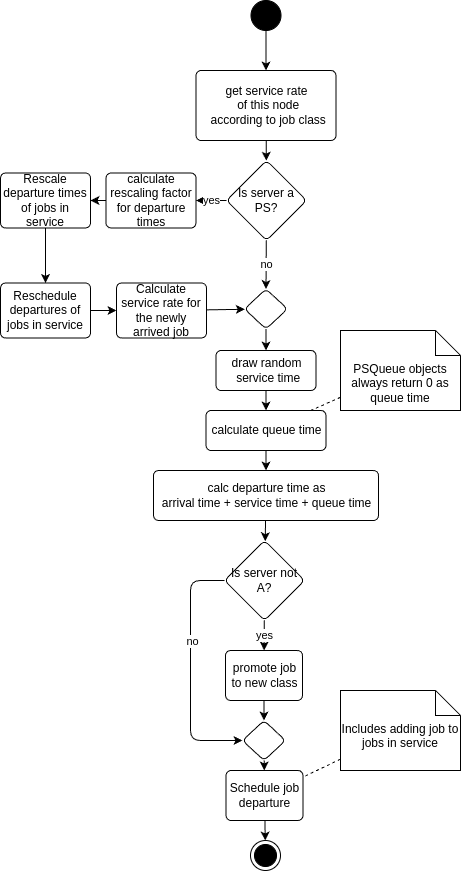
\includegraphics[width=1\linewidth]{figs/diagrams/handle_arrival.drawio.png}
    \caption{Activity diagram dell'handler degli arrivi.}
    \label{fig:handle_arrival}
\end{figure}

\subsubsection{Arrivi e Partenze dei jobs}
\autoref{fig:handle_arrival} mostra i passaggi da intraprendere per gestire l'evento di arrivo di un job a un nodo. In sintesi, l'handler calcola il tempo di departure del nodo come la somma dei seguenti tempi:
\begin{itemize}
    \item Arrival time: tempo di simulazione all'istante di arrivo del nodo;
    \item Service time: tempo che il job deve spendere in servitura, estratto casualmente dalla distrubuzione dei servizi del nodo con parametri che dipendono dalla classe del job;
    \item Queue time: tempo che il job spende nella coda del nodo, che dipende dalla politica di scheduling e dai jobs residenti nel nodo.
\end{itemize}
Nel caso in cui la politica di scheduling sia PS è necessaria particolare attenzione, infatti il ricambio di jobs residenti nel nodo implica un aggiornamento dei tempi di servizio dei jobs già in servitura. Se chiamiamo $S_{rem}$ il tempo di servizio rimanente per un certo job con $N$ jobs in servitura nel nodo otteniamo \autoref{eq:s_rem_ps}, dove $D_{rem}$ è la domanda rimanente da smaltire per completare il servizio su quel job.
\begin{equation}
  \begin{aligned}
    S_{rem} = \frac{D_{rem}}{\frac{\mu}{N}}
  \end{aligned}
  \label{eq:s_rem_ps}
\end{equation}
Nel momento in cui arriva un nuovo job nel nodo, il suo tempo rimanente andrebbe ora calcolato come in \autoref{eq:s_rem_star_ps}, dove $N^*$ è il nuovo numero di jobs nel nodo che include il nuovo job arrivato.
\begin{equation}
  \begin{aligned}
    S^*_{rem} = \frac{D_{rem}}{\frac{\mu}{N^*}}
  \end{aligned}
  \label{eq:s_rem_star_ps}
\end{equation}
Si noti come $D_{rem}$ sia ovviamente la stessa quantità sia in \autoref{eq:s_rem_ps} che in \autoref{eq:s_rem_star_ps}. Mettendo a sistema le due equazioni otteniamo \autoref{eq:s_rem_star_final_ps}, dove $\frac{N^*}{N}$ è il Rescaling Factor menzionato in \autoref{fig:handle_arrival}.
\begin{equation}
  \begin{aligned}
    S^*_{rem} = S_{rem} \frac{N^*}{N}
  \end{aligned}
  \label{eq:s_rem_star_final_ps}
\end{equation}
Usando \autoref{eq:s_rem_star_final_ps} è possibile aggiornare i tempi delle partenze dei job già in servizio nel nodo nel momento in cui arriva un nuovo job. L'effetto che si ottiene è che con l'arrivo di nuovi job, i tempi di servizio rimanente si allungano. Nel caso particolare in cui il job arrivi in un nodo vuoto, allora sia $N$ che $N^*$ sono pari a 1.

\autoref{fig:handle_departure} mostra l'Activity Diagram dell'handler che gestisce la partenza di un job da un nodo. Essenzialmente, rimuove il job dall'insieme dei job residenti al nodo in questione, e se necessario genera un nuovo evento di arrivo al nodo di destinazione. Se il nodo ha politica PS è necessario aggiornare le departures dei nodi ancora residenti usando sempre \autoref{eq:s_rem_star_final_ps}, con l'effetto di accorciare i tempi di servizio rimanenti.

\begin{figure}
    \centering
    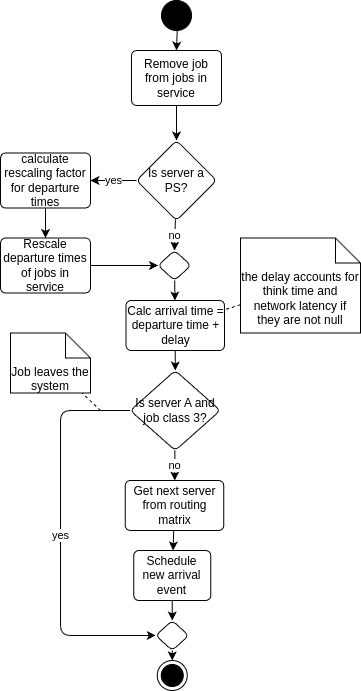
\includegraphics[width=1\linewidth]{figs/diagrams/handle_departure.drawio.png}
    \caption{Activity diagram dell'handler delle partenze.}
    \label{fig:handle_departure}
\end{figure}

\subsubsection{Event-Oriented Programming}
È possibile iscrivere degli \\ \texttt{EventHandler} alla ricezione di uno o più tipi di eventi poiché lo scheduler implementa un pattern Pub-Sub push-notify. L'iscrizione agli eventi può avvenire attraverso i seguenti metodi dello scheduler:
\begin{itemize}
    \item \texttt{subscribe(event\_type, event\_handler)}: l'\texttt{EventHandler} viene invocato dopo che l'evento è stato elaborato, ovvero il suo handler ha terminato l'esecuzione;
    \item \texttt{intercept(event\_type, event\_handler)}: l'\texttt{EventHandler} viene invocato prima che l'evento è stato elaborato, e può modificare l'\texttt{Event} stesso.
\end{itemize}
Non c'è garanzia sull'ordine della ricezione delle notifiche tra subscribers e tra interceptors. Inoltre, iscriversi a un tipo di \texttt{Event} comporta la ricezione delle notifiche anche per eventi che specializzano quel tipo di eventi. Ad esempio, iscriversi al tipo \texttt{Event} implica la ricezione di una notifica ad ogni evento processato. Gli eventi annullati non comportano l'invio di notifiche.

A supporto della realizzazione delle simulazioni sono stati implementati i seguenti subscribers e interceptors:
\begin{itemize}
    \item \texttt{BatchMeansInterceptor}: Intercetta eventi di arrivi esterni per tenerne il conto. Se il conteggio supera il numero di arrivi previsto per il batch, salva le statistiche finora calcolate per questo batch e ripristina le statistiche cacolate dagli stimatori per il prossimo batch.
    \item \texttt{ArrivalsGeneratorSubscriber}: Si mette in ascolto di arrivi esterni e ne tiene il conto. Per ogni arrivo ricevuto, schedula un nuovo arrivo esterno dopo un tempo di interarrivo casuale, fino a quando gli arrivi contati superano il numero massimo di arrivi previsto.
\end{itemize}

\subsubsection{Misurazione metriche di performance}
Gli stimatori delle misurazioni delle metriche di performance sono stati implementati come subscribers e sono i seguenti:
\begin{itemize}
    \item \texttt{BusytimeEstimator}: Si mette in ascolto di arrivi e partenze dei job. Per ogni nodo, traccia gli arrivi e le partenze e tiene conto del numero di jobs ancora presenti nel nodo. Se a causa di un arrivo tale numero passa da zero a maggiore di zero, l'istante di tempo di tale arrivo segna l'inizio di un busy period per quel nodo, che terminerà solo quando tale numero scende di nuovo a zero, oppure lo stimatore è resettato (i.e. quando cambia il batch);
    \item \texttt{ObservationTimeEstimator}: Si iscrive a tutti gli eventi e tiene il conto del tempo di simulazione trascorso dalla sua iscrizione o dal suo ultimo reset;
    \item \texttt{CompletionsEstimator}: Si iscrive alle partenze dei jobs dai nodi. Per ogni nodo,
    conta il numero di partenze dall'inizio della simulazione o dal reset dello stimatore;
    \item \texttt{ResponseTimeEstimator}: Si iscrive agli arrivi e alle partenze dei jobs. Per ogni nodo, si segna il tempo di arrivo e di partenza di ogni job e ne calcola il tempo di risposta come la differenza dei due valori.
    \item \texttt{PopulationEstimator}: Si iscrive agli arrivi e alle partenze dei jobs. Per ogni nodo, ne incrementa il conteggio della popolazione dei jobs per ogni arrivo ricevuto e la decrementa per ogni partenza.
\end{itemize}

Gli stimatori \texttt{ResponseTimeEstimator} e \texttt{PopulationEstimator} mantengono una media dei valori campionati usando un oggetto \texttt{WelfordEstimator}, che implementa l'algoritmo di Welford per il calcolo online della media \citep{des}. Inoltre, tale oggetto calcola anche la Standard Deviation, il Min value e il Max value dei campioni raccolti durante una run. Gli altri stimatori mantengono invece la somma dei campioni.

\begin{figure*}
    \centering
    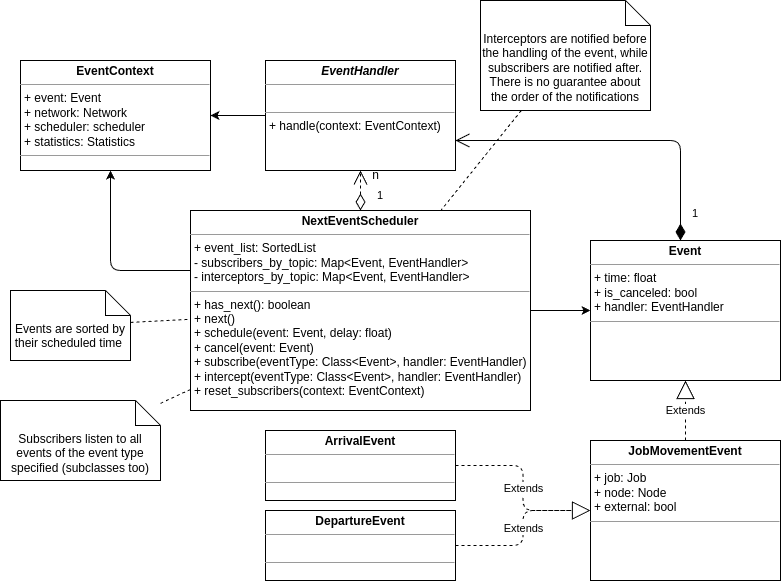
\includegraphics[width=\linewidth]{figs/diagrams/scheduler.drawio.png}
    \caption{Vista delle classi che implementano uno scheduler Next-Event.}
    \label{fig:scheduler_nextevent_class_diagram}
\end{figure*}

\subsubsection{Modello}
\autoref{fig:simulation_class_diagram} mostra come il modello a rete di code è implementato nel sistema. Un oggetto \texttt{Network} si compone di diversi \texttt{Node}, ognuno dei quali è composto da un \texttt{Server} e da una \texttt{Queue}. Il \texttt{Server} implementa il servente e attraverso il metodo \texttt{get\_service(service\_rate)} genera un tempo di servizio casuale secondo un certo rate e distribuzione di probabilità, dopo aver selezionato lo stream corretto. La \texttt{Queue} calcola il tempo che un job deve spendere in coda prima che sia il suo turno di essere servito in base alla politica di scheduling. I tempi di interrarrivo esterni sono calcolati dalla \texttt{Network} secondo la sua distribuzione di probabilità degli arrivi e il rate medio di arrivi.

\subsubsection{Processi stocastici}
La simulazione dei processi casuali è stata implementata usando il modulo \texttt{rngs} \citep{des}, il quale mette a disposizione diversi streams di generatori di Lehmer in grado di produrre una sequenza di numeri pseudo-casuali secondo una distribuzione desiderata. Per ogni processo casuale indipendente simulato nel sistema è selezionato uno stream dedicato, ovvero si imposta il seed del generatore al valore corrente per quello stream prima di pescare il prossimo numero della sequenza. I processi pseudo-casuali indipendenti implementati nel sistema sono:
\begin{itemize}
    \item Gli arrivi dall'esterno del sistema al server A;
    \item I servizi del server A;
    \item I servizi del server B;
    \item I servizi del server P;
\end{itemize}

\begin{figure*}
    \centering
    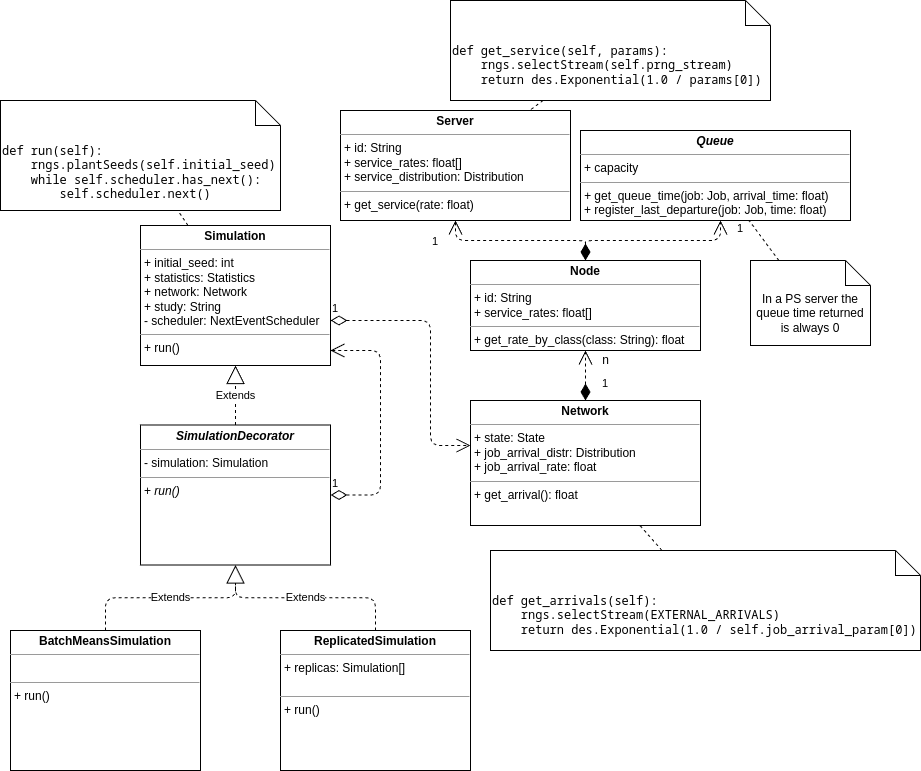
\includegraphics[width=\linewidth]{figs/diagrams/simulation.drawio.png}
    \caption{Vista delle classi che implementano una Simulazione.}
    \label{fig:simulation_class_diagram}
\end{figure*}

\subsubsection{Simulation Runs}
Una simulazione è implementata come un oggetto \texttt{Simulation}, come illustrato in \autoref{fig:simulation_class_diagram}. Attraverso l'uso di decoratori, sono state implementate due varianti di simulazione:
\begin{itemize}
    \item \texttt{BatchMeansSimulation}: Iscrive alla simulazione decorata un \texttt{BatchMeansInterceptor} per implementare una simulazione Batch Means;
    \item \texttt{ReplicatedSimulation}: Decora una sequenza di simulazioni identiche e le esegue in sequenza, impostando il seed iniziale della prossima replica come l'ultimo valore della sequenza prng (\texttt{DEFAULT} stream) generato dalla replica precedente.
\end{itemize}
È possibile implementare una run di simulazione aggiungendo a runtime i comportamenti desiderati utilizzando opportunatamente decoratori, subscribers e interceptors, oltre a costruire la rete di code desiderata andando a comporre opportunamente oggetti \texttt{Server} e \texttt{Queue} in oggetti \texttt{Node}, e questi ultimi in una \texttt{Network} da associare poi alla \texttt{Simulation}. Inoltre, è necessario impostare un evento iniziale che di fatto dà il via alla simulazione. Nel nostro caso, abbiamo delegato la complessità della costruzione di una simulazione in una \texttt{SimulationFactory}. Queste caratteristiche rendono il simulatore molto potente e flessibile in termini di features mantenendone contenuta la complessità della implementazione.   

Una volta costruita una \texttt{Simulation}, per eseguirla è sufficiente invocarne il metodo \texttt{run()}, che imposta il seed iniziale per i vari streams del prng e avvia la consumazione degli eventi. Quando non ci sono più eventi da consumare, la simulazione termina e viene effettuato il salvataggio delle statistiche su dei file \texttt{.csv} nella cartella \texttt{statistics}. I parametri della simulazione sono definiti in un file \texttt{config.json}, dove a ogni entry corrisponde un set di valori di parametri che realizzano un Simulation Study.
